\chapter{Sparse Field - Implemented code}
\section{Introduction}
The sparse field level set method was implemented in C++ for the project, and the implemented code is mainly based on the pseudocode in \cite{lankton09}, which again is based on Whitaker's introduction to the sparse field method in \cite{whitaker89}. 
The sparse field was first implemented in 2D and after bugfixing and some test-runs it was extended to 3D, which is executed in the exact same was as the 2D version. Both the 2D and 3D versions of the implemented code can be found in appendix B, and the pseudocode (only in 2D) can be found in appendix A. In this chapter the pseudocode in \cite{lankton09} will be explained first, along with how it works. Secondly, the differences between Lankton's pseudocodes in \cite{lankton09} and the implemented code will be described. And finally there will be a detailed explanation of the implemented code.

\section{TODO}
As previously mentioned, the sparse field method can be implemented using linked lists to hold the pixels being used in the calculations. Pixels in this context does not mean the pixels in the original or segmented image, but the points in the matrix that represents the $\phi$. These pixels are seperated into five layers, each represented by a linked list. One of the lists holds the active points, i.e the zero level set, and is referred to as the Lz list. The rest of the needed pixels are seperated according to their closeness to the pixels in Lz and which side of the Lz pixels they are located. The Ln1 list contains the pixels that are adjacent to Lz pixels on the inside of the object being segmented. Similarly Lp1 contains pixels that are adjacent, but on the outside. All pixels that are adjacent to those in Ln1 except for those in Lz are elements in the Ln2 list, and similarly the ones adjacent to Lp1 on the opposite side of Lz are part of Lp2. This becomes more clear when looking at table \ref{rangeTab1} and figure \ref{labelExample}. 

\begin{table}[h] %h = here
	\begin{tabular}{| c | c |} 
	% l = left-justified columns, alternatives are: r (right) and c (center)
	% | = vertical line, \hline = horizontal line
	\hline
	List Name & Range\\
	\hline
	Lz & [-0.5, 0.5]\\
	Ln1 & [-1.5, -0.5>\\
	Lp1 & <0.5, 1.5]\\
	Ln2 & [-2.5, -1.5>\\
	Lp2 & <1.5, 2.5]\\
	\hline
	\end{tabular}
	\caption{Range of lists used in \cite{lankton09}}
	\label{rangeTab1}
\end{table}

\begin{figure}[h!]
\centering

\includegraphics[width=0.65\textwidth]{implemented/labelExample}
\caption{Label image: image showing the different layers under segmentation.}
\label{labelExample}
\end{figure}

Figure \ref{labelExample} represents the 5 different layers with different colors. The black colored part is defined to be inside the object being segmented, the white part as outside, and these two parts are not used in the computation for the current iteration. The dark blue pixels around the dark part are the pixels contained in Ln2, and the brown pixels are those on Ln1. The dark-purple colored pixels are Lz elements, light-purple are Lp1 and light-blue are pixels in Lp2. This type of image will henceforth be referred to as the $label$ image, because it shows the labels of the image being segmented.

\section{Forskjeller fra vår kode og pseudokoden til lankton}
Some improvements and changes from Lankton's pseudocode were made
By looking closer at table \ref{rangeTab1} it can be seen that Lz has a slightly wider ramge than the other lists. This range of exactly 1 causes in some cases huge problems that lead to disortions and artifacts in the segmentation. What these problems are will be discussed in LINK TIL DET HER. To overcome these problems the ranges of the lists were slightly changed to make all the lists equal in range. The range-corrected lists are shown in table \ref{rangeTab2}, and even though the change seems insignificant it actually does change the result significantly (as will be discussed in SAMME LINKEN HER).

\begin{table}[h] %h = here
	\begin{tabular}{| c | c |} 
	% l = left-justified columns, alternatives are: r (right) and c (center)
	% | = vertical line, \hline = horizontal line
	\hline
	List name & Range\\
	\hline
	Lz & [-0.5, 0.5>\\
	Ln1 & [-1.5, -0.5>\\
	Lp1 & [0.5, 1.5>\\
	Ln2 & [-2.5, -1.5>\\
	Lp2 & [1.5, 2.5>\\
	\hline
	\end{tabular}
	\caption{Range of lists used in the implementation}
	\label{rangeTab2}
\end{table}

\section{Om koden vår}
\subsection{Datastructures and types used - elr noe lignende}
In addition to the five lists representing the as five layers, two arrays of equal size and dimension as the image to be segmented are used. One of them is the $label$ image described above, which is used to track where the pixels containing the different layers are on the domain. Given a pixel, to find out which layer (if any) that pixel is a member of, a simple lookup to the $label$ is enough. Another excellent feature of the $label$ array is that it can be used to verify that all the layers are correclty aligned and if there are any pixels of any layers that are poorly placed. The $label$ image can thus be used to find artifacts that might have resulted from code errors. An example of a $label$ image (zoomed in to be able to clearly see the artifacts) which clearly states that there is something wrong with how the layers are handled in the code is shown in figure \ref{labelFailedEx}. How the $label$ label image actually should have been is illustrated in figure \ref{labelOkEx}.

\begin{figure}[h!]
\centering

\includegraphics[width=0.90\textwidth]{implemented/labelFailedEx}
\caption{A label image with pixels in places they should not be.}
\label{labelFailedEx}
\end{figure}

\begin{figure}[h!]
\centering

\includegraphics[width=0.90\textwidth]{implemented/labelOkEx}
\caption{How the label image should have been.}
\label{labelOkEx}
\end{figure}

The other array used is the $\phi$ - array, which contains the actual $\phi$ values of each pixel in the domain. The range of the values is exactly the same as in the $label$ image, but while the $label$ image only contains integer values describing which layer a pixel is part of, the $\phi$ image contains the actual values (floating point numbers) of the level set. The images represented by the $label$ and $\phi$ arrays would thus be very similar (though small differences may be seen) when looking at, but they do have different tasks. The $label$ is as mentioned used as a lookup table, while the $\phi$ array determines which layer a pixel belongs to after its pixels have been updated with the speed function.

To correctly move pixels between the layers some temporary lists have to be used, one for each layer. By using these temporary lists, called Sn2, Sn1, Sz, Sp2 and Sp2, pixels are prevented from being moved more than 1 layer at a single iteration. Assume that pixel $A$ is in Ln1 and has two neighbours in Lz. These two neighbours will be updated by the speed function and may move out of Lz into either Ln1 or Lp1. If both these pixels are moved out of Lz, pixel $A$ will no longer have any neighbours in Lz and will in most cases be incorrectly moved to Ln2. This is only of of many possible mistakes that could happen when not using temporary lists, an another example is that a pixel could be moved to a list and then back to where it came from within the same iteration. Using temporary lists prevent such problems by adding the pixels that are to change layer into them, removing the pixels from the original lists, and finally when all temporary lists are filled with pixels to be moved and all the original lists have the pixels moving out of them removed, then the original lists are filled with those in the temporary lists. And then the temporary lists are emptied before the next iteration starts.


FLYTT dette vekk til et annet sted...................
Before explaining what this means, a brief look into how the pixels are pushed to and popped from the different lists is needed. First the speed function is calculated for each pixel in Lz (will be explained in more detail in LINK TIL DER SPEED FUNCTION BLIR FORKLART). Then the four remaining lists are updated, but not using the speed function as with the Lz pixels. Since Ln1 and Lp1 are defined to be neighbours to Lz on each side, and Lp2 and Ln2 as neighbour to Lp1 Ln1 respectively, there is no need to use computation time to calculate their speed function. They will follow Lz, e.g. if a pixel in Lz moves to the right, then its neighbours (in Ln1 and Lp1) at each side will also move a step to the right. Similarly Ln2 and Lp2 pixels will follwow Ln1 and Lp1 respectively. How this actually is implemented is described in LINK HER

\subsection{Code structure}
The code is seperated into two C++ files, main.cpp and update.cpp, and two corresponding header files. The update.cpp file consist of everything that happens at each iteration, this icnludes calculating the speed function, updating the $\phi$ - array with the speed, updating the $label$ array and update the lists. The main.cpp file consist of actions that are executed before and after the actual segmentation, such as initializing everything, handle input and reading/writing to/from the input image and segmentation result. 

\subsection{Input and initialization}
TODO skriv om input\\
An array of same size as $label$ and the $\phi$ - arrays is used to initialize $label$, the $\phi$ - array and Lz. This array, called init, is initialized to zero valued elements at start, and then filled with 1's given the x,y (and z in 3D) coordinates along with a radius given as input. These input values creates a circle (or sphere if 3D) of 1's in the init array that represents the seed points. Multiple coodrinates and radiuses can be given as input to create multiple seed points. Based on the values in init the two arrays $label$ and $\phi$ are initialized. All pixels in $label$ and $\phi$ corresponding with the ones in init with value 1 are set to -3 to indicate that they are inside the segmentation object. All other pixels in $label$ and $\phi$ are set to 3 indicating that they are outside the object. Then the corresponding pixels to all values in init that are 1 but have 0 valued neighbours are set to 0, indicating that they are part of the zero level set. Then these pixels are added to Lz as initial zero level set values. Then $Ln1$, $Lp1$, $Ln2$ and $Lp2$ are filled according to their definitions, and the $label$ and $\phi$ arrays are updated to refelct these changes. After these initializing actions are finished the segmentation process can start. 
The $\phi$ - array is initialized by the using the x,y (and z in 3D) coordinates along with the radius to create a circle. This circle is 

\subsection{Speed function explained}
Two different speed functions are implemented. These are seperatly implemented in their own methods, and a speed function is only referenced in one place in the code. This makes it easy to implement new speed functions, and to change between which of them to use when running the program. The speed function methods takes in as parameters the coordinates of the pixel to calculate the speed chnage on, and returns a value which then is added to the speed from the last iteration. The two speed functions are implemented are the one explained in chapter \label{levelSetChap} and a much more simple one based on the Chan-Vese energy. Simply put, the Chan-Vese energy ($E^{CV}$) is defined as 
\begin{equation}
E^{CV}(c_1,c_2,C) = \int_{inside(C)} (\mu (x,y) - c_1)^2 \, dx \, dy \, + \, \int_{outside(C)} (\mu (x,y) - c_2)^2 \, dx \, dy \, \cite{wang10} %\, = whitespace
\end{equation}
where $\mu$ is the image, and C is a closed segmentation curve which in this case is the curve defined by the zero level set. The constants $c_1$ and $c_2$ are the average greyscale intensity values inside and outside of C, respectively. Discretizing this energy function, and writing it as a pixelwise function gives
\begin{equation}
E^{CV}(x,y) = (\mu (x,y) - c_1)^2 - (\mu (x,y) - c_2)^2
\end{equation}
TODO forklar litt om hvordan denne speed funksjonen virker\\
Husk også å nevne at return verdien må være i intervallet <-1,1> og hvorfor.

\section{Problems met}
As previously mentioned, when looking at figure \ref{labelFailedEx} it can be clearly seen that something is wrong with how the lists (the layers) are arranged. This becomes even more clear when looking at figure \ref{failedZeroEx} which shows only the zero level set.
\begin{figure}[h!]
\centering
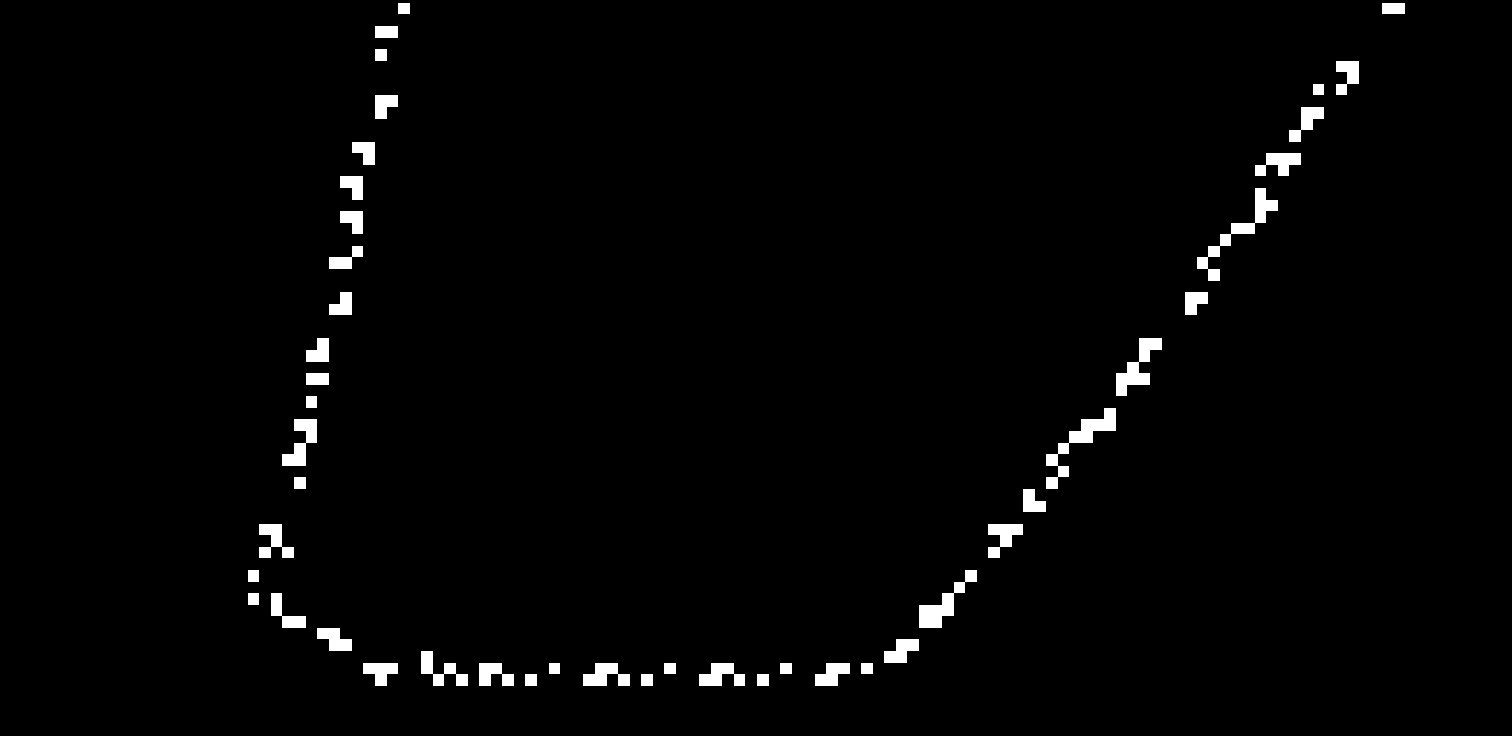
\includegraphics[width=0.90\textwidth]{implemented/failedZeroEx}
\caption{Zero level set corresponding to the label image in figure \ref{labelFailedEx}.}
\label{labelOkEx}
\end{figure}
The zero level set in figure \ref{failedZeroEx} is the segmentation result (zoomed in) that corresponds to the label image in figure \ref{labelFailedEx}. The zero level set is supposed to be a one pixel wide continous line, but in this case that is not true. Several problems and bugs in the code combined were reasons were for this result. Much time and effort was used to debug this and to fix these problems. In addition to creating artifacts in the results, the bugs also made the program run much slower which made the debugging process even more time consuming. The main problem was that the speed function was not normalized to be within the range $<-1,1>$, which triggered the problems mentioned in the previous section(TODO: Husk å skrive om problemene i Speed function explained subsectionen). Another thing that caused problems was a bug in the code that in some cases moved a pixel from $Lp1$ to $Ln2$ when it was supposed to move to $Lp2$. This bug occured only in the 3D implementation and only under certain circumstances, which made the debugging process more complicated and cumbersome. MER??


Figures X2 and X3 depicts the segmentation result of the same original input image with equal number of iterations completed, with the ranges from table  \ref{rangeTab1} and \ref{rangeTab2} used resprectively. Som vi ser så ser X3 mye bedre ut blabalba, pga endringene in the ranges of the lists
....

\section{Performance}
Both C++ and Matlab were candidates languuages to implement the level set function in. The adavatage of using Matlab is the simple syntax used for mathematical operations and the ease of loading/writing and displaying images in both 2D and 3D. But ultimately C++ was chosen because of its advantages in speed and the possibility of parallelization.
Several improvements to increase the performance were made after a working 3D version was complete, some which gave insignificant or small performance increases, and a few which greatly improved runtime. One of the changes made to achieve significantly improved runtime was as simple as changing all structures defined as $double$ to $float$. In many cases this change may seem insignificant, but in this case with data structures of sizes as big as $256^3$ and several linked-lists with hundreds of pixels being pushed and popped each itereation, the change reduced the runtime by ???? in 2D and ??? in 3D. (TODO finn ut hvor raskere segmenteringen kjørte etter double til float endringen) A chance that imroved the runtime even more significanly was the replacement of the C++ datastructure $std::vector$ with the datastructure $std::list$. When the implementation process started $std::vector$ was chosen as the container for the elements in the different layers, without considering any other candidates. The runtime in 2D using $vwctor$ was not considered slow, hence vector was also used for 3D. But due to the slow speed of the 3D version (when using $vector$) changes were needed. One improvement was the above-mentioned double to float change, and using $list$ instead of $vector$ was the second significant change. Some of the advantages and disadvantages of using the $std::list$ and $std::vector$ are summarized in table \ref{vectorTab} and \ref{listTab}.

\begin{table}[h!]
	\begin{tabular}{| p{5.5cm} | p{5.5cm} |} 
	\hline
	\multicolumn{2}{|c|}{Vector} \\
	\hline
	Advantages & Disadvantages \\
	\hline
	Efficient accessing of its elements & Cannot access element $m$ ($1<m<n$) directly: must iterate through 1 to $m-1$ to get to $m$. \\
	Insertion/erasure from the end uses constant time &  Insertion/erasure from other than end is costly (O(n)) \\
	\hline
	\end{tabular}
	\caption{Advantages and disadvantages of C++ $std::vector$}
	\label{vectorTab}
\end{table}

\begin{table}[h!]
	\begin{tabular}{| p{5.5cm} | p{5.5cm} |} 
	\hline
	\multicolumn{2}{|c|}{List} \\
	\hline
	Advantages & Disadvantages \\
	\hline
	Fast insertion, extraction and moving of elements in any position & Consume some extra memory to keep the linking information associated to each element \\
	\hline
	\end{tabular}
	\caption{Advantages and disadvantages of C++ $std::list$}
	\label{listTab}
\end{table}
The reason for the drastical inmprovement in performance when changing from $vector$ to $list$ is because of the overhead when using $vector$ associated with inserteion and erasure of elements not at the end. After the first few iterations, these two actions happens hundreds of times per iteration, and by changing to $list$ this overhead along with the smaller $log(n)$ overhead when increasing the size of the vector is eliminated, which improves performance and speed. The speedup gained by changing the element types from using double to float and the speedup aquired when replacing $vector$ with $list$ is shown in table \ref{speedUps}.

\begin{table}[h!]
	\begin{tabular}{ c | c | c | c | c |} 
	\cline{2-5}
	 & \multicolumn{2}{|c|}{double \rightarrow float} & \multicolumn{2}{|c|}{vector \rightarrow list}\\
	\cline{2-5}
	 & 100 iteration & full segmentation & 100 iteration & full segmentation  \\
	\hline
	\multicolumn{1}{ |c| } {2D} & TODO & X2 & X3 & X4  \\
	\hline
	\multicolumn{1}{ |c| }{3D} & X1 & X2 & X3 & X4  \\
	\hline
	\end{tabular}
	\caption{Runtime improvements in 2D and 3D.}
	\label{speedUps}
\end{table}

To speed up the process even more some parts of the code were run in parallel by using OpenMP. OpenMP is an API that supports shared memory multiprocessing in C, C++ and Fortran. OpenMP was used even before $vector$ was replaced with $list$, and was chosen because it only reguires a few well placed lines of code. OpenMP was implemented right after the first 3D version was completed, and was used to speed up the process when different datasets were used as input to compare the results against each other (TODO: Dette avsnittet må forbedres).
Another change that was considered but later dropped, was to replace the use of $list$ with $std::forward_list$. This structure was considered due to its slightly less overhead when inserting and removing elements which makes it more efficient than $list$. But this improvement in insertion and deletion time over $list$ comes as a consequence of the fact that $forward_list$ is a single linked list, and is thus not able to point to the previous element in the list. The sparse field level set methd can be implemented using single-linked lists instead of double-linked lists, but the implementation in this project depends on the lists being double-linked, so to being able to use single linked lists a complete makeover of the code is necessary, which due to the scope of time was not an option.


